\chapter{Konzeption}

Bevor mit der Entwicklung selbst angefangen werden kann, sollte zuerst das
Konzept für die Applikation erstellt werden. Dies beinhaltet verschiedene
Aspekte, wie die Planung des Projektes selbst, die Konzeption der
Funktionalität der Applikation und die Technologien und Tools für die
Entwicklung. Die folgenden Abschnitte sollen diese drei Beschriebenen Punkte
genauer beleuchten.

\section{Projektplanung}

Das Projekt wurde alleine ohne ein Team entwickelt. Obwohl bei einer Arbeit
alleine viel mehr Freiheiten offen sind als bei einer mit einem Team, sollte
generell nicht ohne Struktur gearbeitet werden. Eine Festlegung einer
Arbeitsweise verhilft dabei ein großes Projekt in kleine bearbeitbare
Arbeitspakete aufzuteilen und diese systematisch bearbeiten zu können.

Für die Bearbeitung dieses Projektes wurde hierfür eine einfache, agile
Arbeitsweise gewählt. So sollte das Projekt iterativ entwickelt werden, um
schnell im Projekt einen arbeitsfähigen Prototyp zu erhalten. Hierfür sollten
Arbeitspakete erstellt werden, welche jeweils ein einzelnes, abgeschlossenes
Feature erhalten. Ein solches Arbeitspaket kann \zb{} die Nutzerverwaltung sein.
Solche Arbeitspakete können auch Abhängigkeiten untereinander haben, da \zb{}
das Erstellen eines Teams nicht ohne die Nutzerverwaltung möglich ist, ein solches
Team immer an einen Nutzer gebunden ist und so die die Implementierung nicht möglich wäre.
So kann auch eine sinnvolle Bearbeitungsreihenfolge für die
Features bestimmt werden. An diesen Features kann Schritt für Schritt
gearbeitet werden, bis ein \anf{Minimal Viable Product} (MVP) entsteht, mit
welchem einem Nutzer die Kernfunktionalitäten des Produktes gegeben werden. Nach
diesen kann das Produkt weiter mit optionalen Features erweitert werden, die
zwar für die Nutzer einen Mehrwert bieten, jedoch nicht essenziell für die
Funktionalität sind.

Für die Planung eines solchen Projektes stehen dabei viele diverse Tools zur
Verfügung. Um den Mehraufwand für die Projektplanung so gering wie möglich zu
halten, wurde die integrierte Lösung von Gitlab~\cite{gitlab} verwendet. So
können zu den bisher beschriebenen Arbeitspakete \sog{} \anf{Issues} angelegt
werden. So wurde bevor mit der Entwicklung eines solchen Features immer das
jeweilige Issue erstellt, an dem gearbeitet werden sollte.

\section{Funktionalität}

Bevor die Technologien und die Architektur für das Projekt gewählt werden
können, sollte nun das Ziel des Projektes und die Funktionalität dessen
beschrieben werden. Damit können anhand der beschriebenen Anforderungen, besser
die benötigten Technologien gewählt werden. Die folgenden Unterabschnitte
sollen so die benötigten Funktionalitäten beschreiben, welche für eine
Teambasierte Chatapplikation benötigt werden. Da kein separates Design \bzw{} Mockups
für die Funktionalität erstellt wurden, werden die beschriebenen Anforderungen
durch die schon implementierte Software illustriert.

\subsection{Nutzerverwaltung}

Die Nutzerverwaltung stellt eine grundlegende Funktionalität der Applikation
dar, ohne die Teams und deren Unterkomponenten nicht erstellt werden können. Das
wichtigste Ziel dieser ist es, dass neue Nutzer zum einen sich auf der Plattform
registrieren können, als auch bestehenden Nutzern einen Login zur Plattform zu
ermöglichen. Hierfür sollen in beiden Fällen Forms für beide Aktionen dem
Nutzer gezeigt werden, wenn dieser in seinem Browser noch nicht eingeloggt ist.
Die Nutzer können sich, wie es in der Abbildung~\ref{fig:loginForm} gezeigt wird, mit einer
Kombination aus einem Nutzernamen und einem Passwort einen Login ausführen
\bzw{} sich registrieren.

\begin{figure}[ht]
  \captionsetup{justification=centering}
  \centering
  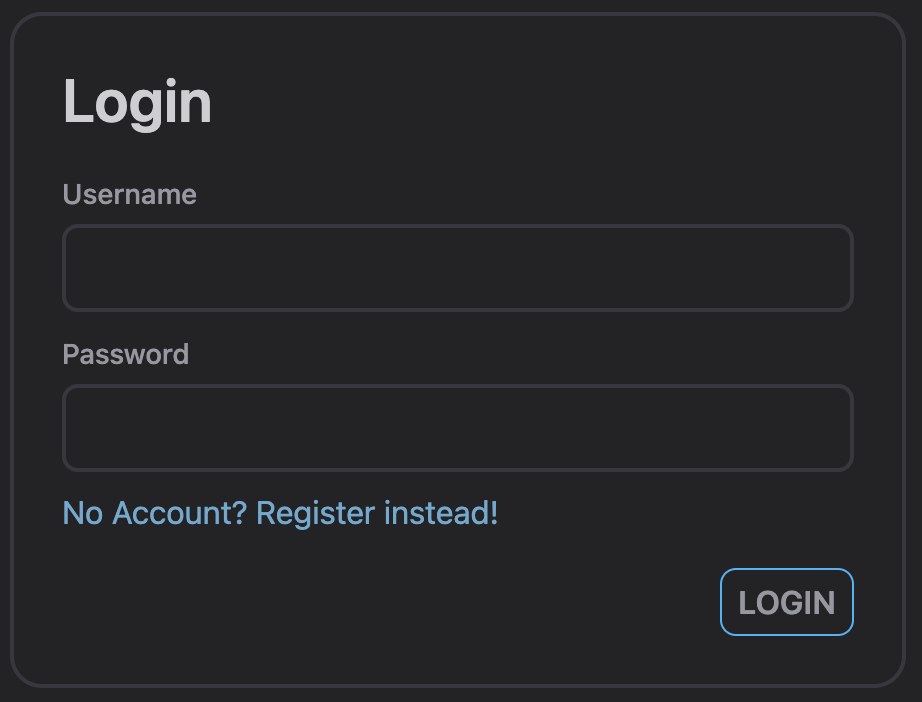
\includegraphics[scale=0.5]{./assets/login.png}
  \caption{Login-Form}\label{fig:loginForm}
\end{figure}

Eine weitere Funktionalität der Nutzerverwaltung ist, dass der Nutzer selbst
Anpassungen an ihrem Account machen können. Da nur sehr wenige Daten über den
Nutzer gespeichert werden, beschränkt dies sich auf drei Aktionen. So kann ein Nutzer
seinen Anzeigenamen für die Chats im Team bearbeiten können, welcher als Standard auf
den Nutzernamen gesetzt ist. Auch sollte es die Möglichkeit geben sein Passwort ändern zu können als auch den
Account endgültig zu löschen, wenn dieser nicht mehr benötigt wird. Diese
Optionen sollten über die Einstellungen zu finden sein.

\subsection{Teams}

Nachdem ein Nutzer in der Plattform eingeloggt ist, sollte dieser nun die
Möglichkeit haben, seine bisher erstellten Teams betrachten zu können und diese
zu verwalten. Hierfür wird zuerst den Benutzer über in einer Seitenleiste
alle seine Teams angeboten, welcher dieser selbst erstellt hat oder welche mit
ihm geteilt wurden. Über ein Modal, dass durch die Seitenleiste erreicht werden kann,
kann der Nutzer beide Aktionen durchführen. Zum Erstellen eines neuen Teams muss nur
der Name für dieses angegeben werden. Wenn einen bestehenden beigetreten werden sollte,
kann dies über einen Invite-Code erreicht werden.

\begin{figure}[ht]
  \captionsetup{justification=centering}
  \centering
  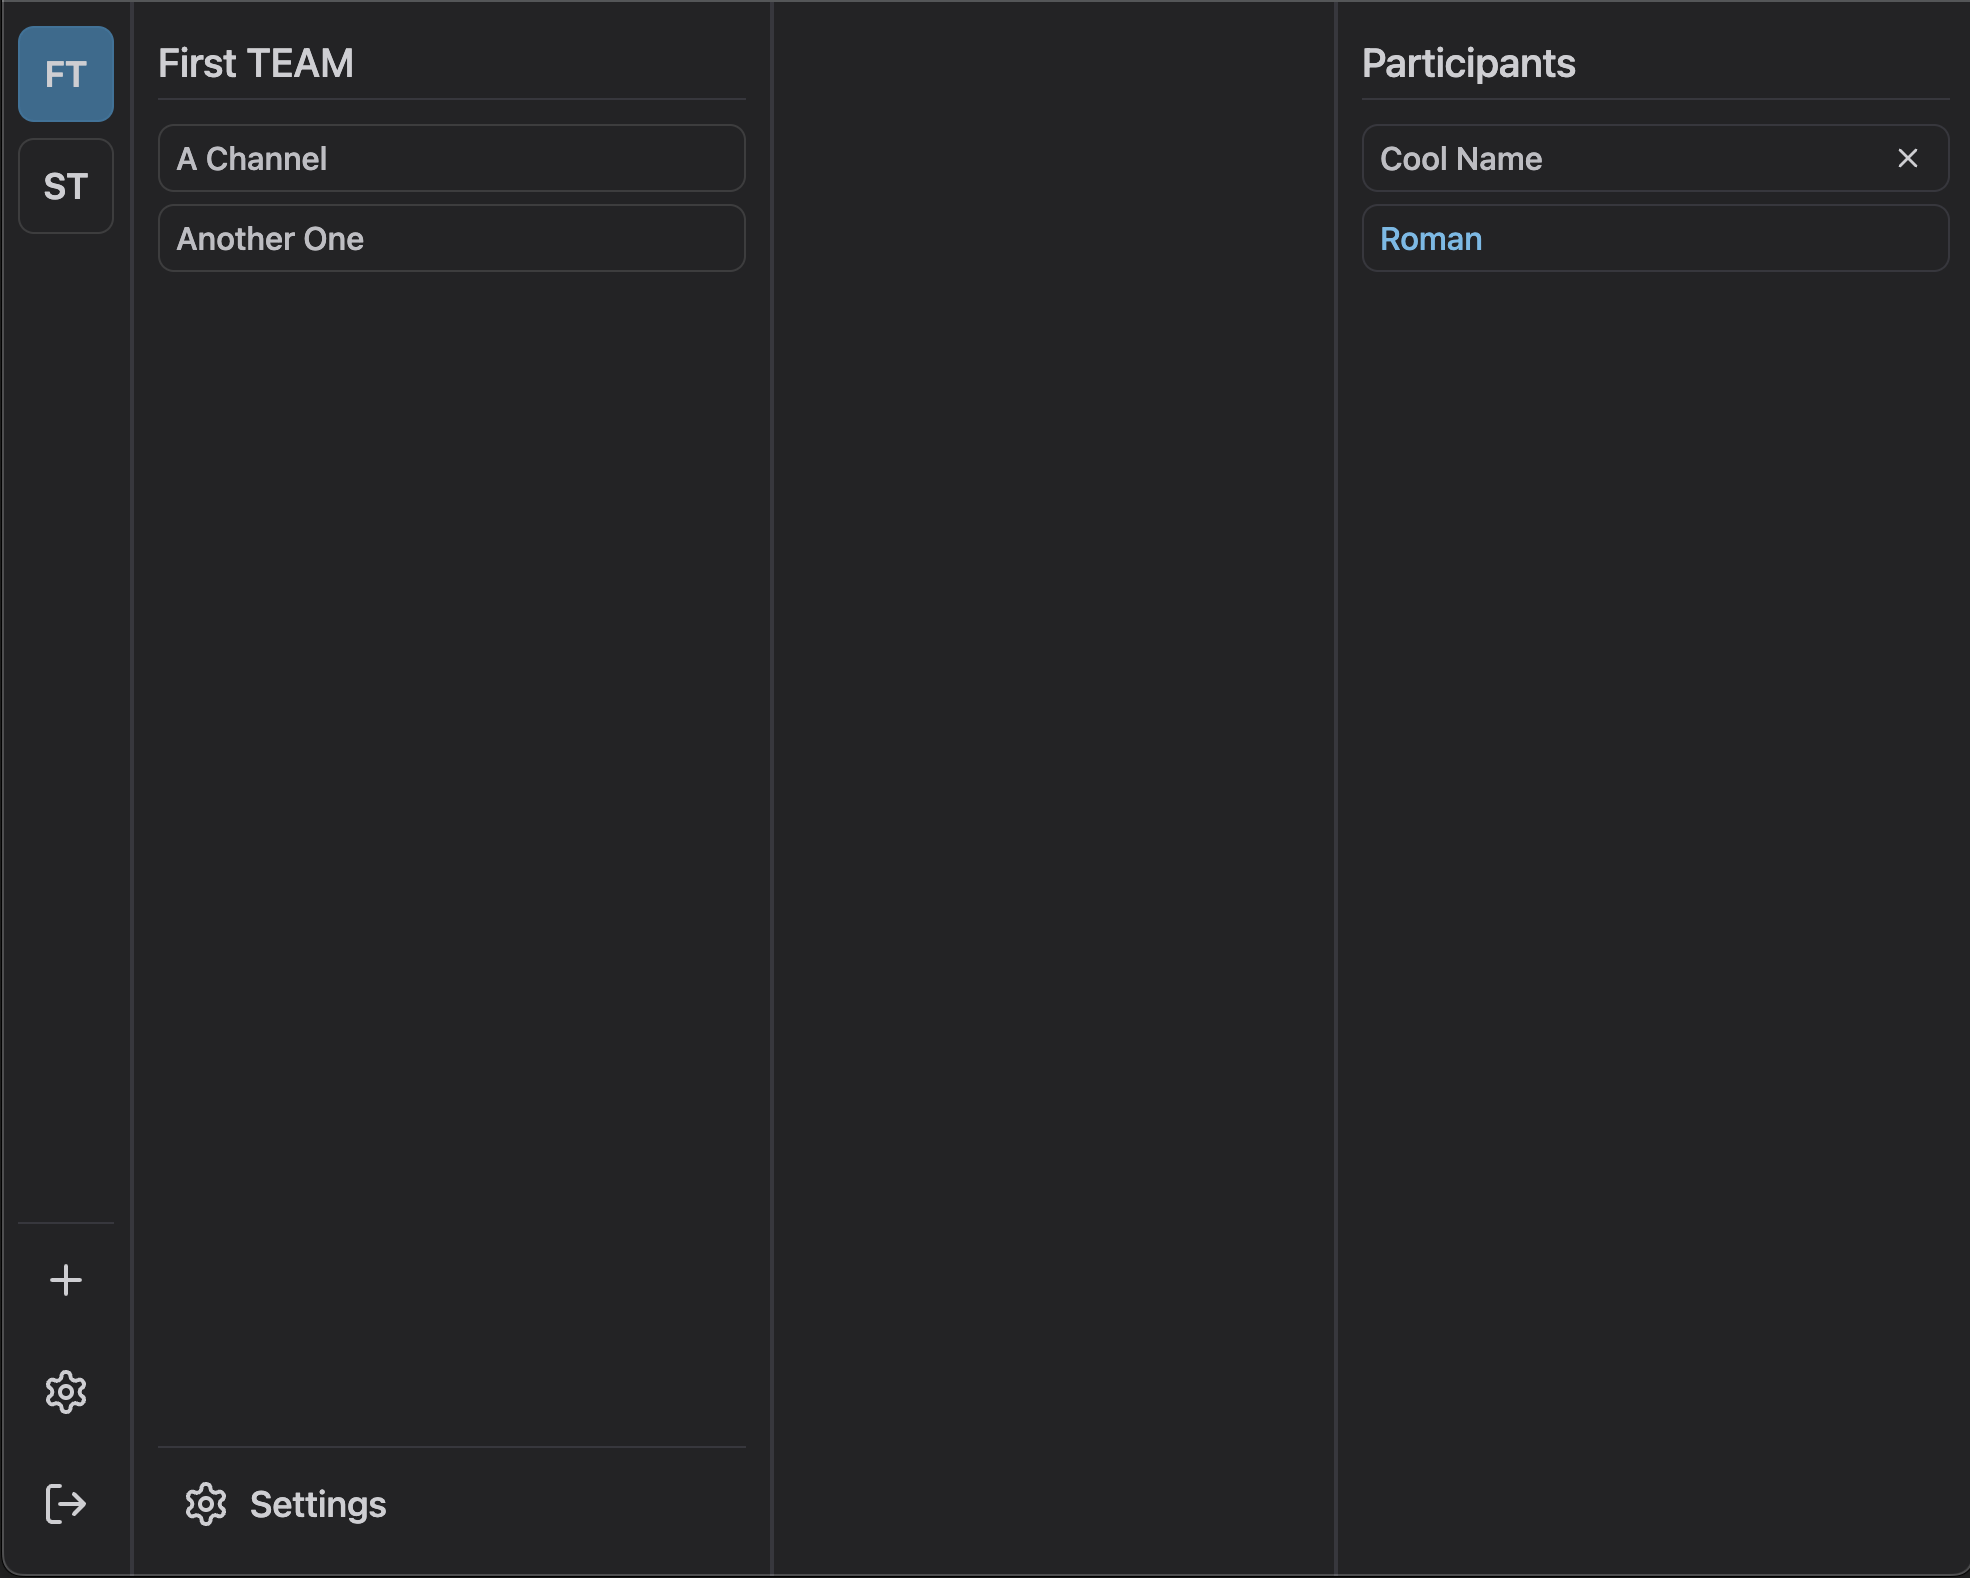
\includegraphics[scale=0.35]{./assets/team_overview.png}
  \caption{Teamübersicht}\label{fig:teamOverview}
\end{figure}

Von der Seitenleiste aus kann zu einem spezifischen Team navigiert werden, wo man zum dem
Hauptinterface der Applikation kommt. Diese ist eine drei geteilte Ansicht, welche die wichtigsten
Informationen für ein Team zeigt. Die Abbildung~\ref{fig:teamOverview} zeigt diese Ansicht. Diese
zeigt die bisher erwähnte Seitenleiste zur Übersicht aller Teams. Neben dieser finden sich zwei weitere
Seitenleisten, die zum Team gehören. In der linken Seitenleiste werden die Textkanäle angezeigt,
welche wenn betreten, visuell markiert werden. Neben dieser erhält der Besitzer des Teams einen Button
zu den Einstellungen eines Teams, während ein eigeladener Nutzer stattdessen einen Button zum Verlassen
des Teams auffindet. In der weiteren Seitenleiste finden sich alle Teilnehmer des Teams. Hier wird
der Besitzer des Teams speziell markiert. Auch erhält der Besitzer des Teams die Möglichkeit
über diese Liste eingeladene Nutzer aus dem Team zu entfernen.

Auch sollte jedes Team seine eigenen Einstellungen haben. In diesen Einstellungen sollen zuerst
allgemeine Optionen zu dem Team verwaltet werden. Dies beinhaltet zum bisherigen Zeitpunkt nur die Option
den Namen des Teams zu ändern. Daneben können hier die Textkanäle verwaltet werden. Dafür kann ein neuer
Kanal hinzugefügt und bestehende gelöscht werden. Die Option bestehende Kanäle nur umzubenennen, gibt es bisher nicht.
Zuletzt sollen hier neue Invite-Codes für das Team generiert werden. Dieser kann der Besitzer des Teams erstellen
und an weitere potentielle Nutzer geben, welche diese dann einlösen können. So ist eine einzelne Einladung nur
einmal gültig.

\subsection{Textkanäle}

Die letzte Funktionalität stellen die Textkanäle, mit den Nachrichten in diesen dar.
Wenn der Nutzer in einem Team zu einem Kanal navigiert, sollte dieser die Möglichkeit haben
einzelne Textnachrichten zu senden und bereits gesendete zu betrachten. Dafür wird ein Chatfenster
im bisher leeren Bereich zwischen den Seitenleisten, wie es in der Abbildung~\ref{fig:chatMessages} zu sehen ist,
im Team gezeigt, wenn auf einen der Kanäle in der Seitenleiste geklickt wird. Danach kann
der Nutzer Nachrichten schreiben, die allen Nutzern zugestellt werden. Wenn der Nutzer eine
Nachricht sendet und weitere Teilnehmer zurzeit denselben Kanal betrachten, wird diese Nachricht
allen Teilnehmern in Echtzeit zugestellt und die Seite muss nicht neugeladen werden. Neben den Echtzeit-Nachrichten kann auch die Historie des Kanales
mit den bisher gesendeten Nachrichten betrachtet werden. Diese sollten, damit der Nutzer nicht zu lange
auf die Historie warten muss, in kleinen Paketen geladen werden. Wenn der Nutzer an das Ende der bisher
geladenen Historie gescrollt hat, sollten diese falls noch Nachrichten vorhanden sind, nachgeladen werden.

\begin{figure}[ht]
  \captionsetup{justification=centering}
  \centering
  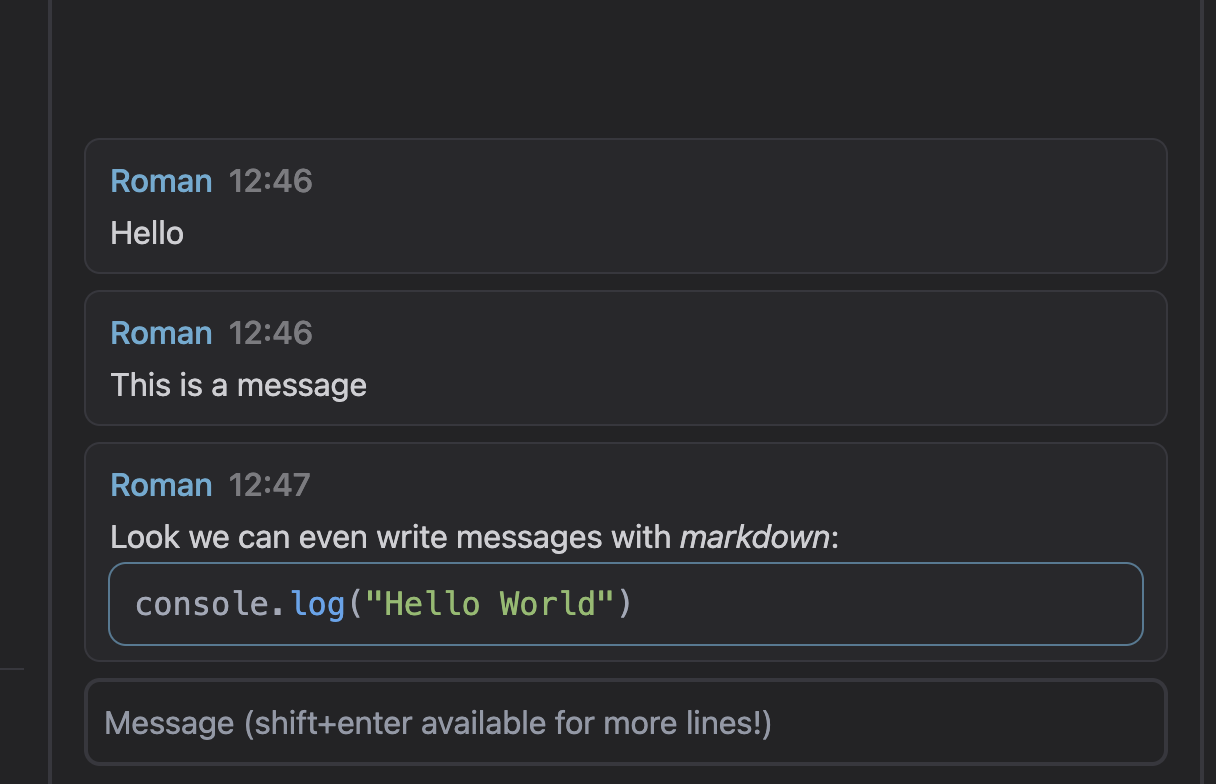
\includegraphics[scale=0.45]{./assets/chat_messages.png}
  \caption{Textkanalnachrichten}\label{fig:chatMessages}
\end{figure}

Um die Nachrichten zu schreiben, wird ein Textfeld angeboten. In diesem sollten die Nachrichten einfach
geschrieben werden und mit dem Drücken der Enter-Taste gesendet werden können. Da öfters auch längere
Nachrichten gesendet werden müssten, kann mit der Kombination aus der Shift- und Enter-Taste eine
neue Zeile begonnen werden. Das Textfeld wird sich hierfür auch automatisch in der Größe erweitern.

\section{Technologien}

Zuletzt sollen noch für die Konzeption die verwendeten Technologien, die
Architektur und das Datenmodell der Applikation beschrieben werden. Diese
sollen zeigen, nach welchen generellen Prinzipien das Projekt aufgebaut wurde.

\subsection{Datenmodell}

Da für dieses Projekt Nutzerdaten persistent gespeichert werden müssen, wird auch
ein Datenmodell für dieses benötigt. Dabei wurde für die persistente Haltung
der Daten sich für eine relationale Datenbank entschieden. Hierfür wurde die
Datenbank PostgreSQL verwendet. Die Abbildung~\ref{fig:dbSchema} zeigt dabei
das Datenbankschema der Applikation. Da die Tabellen im Backend direkt
auf Klassen gemapped werden und der Name beibehalten wird,
haben auch die Tabellen hier eine \anf{Entity}-Endung.


\begin{figure}[ht]
  \captionsetup{justification=centering}
  \centering
  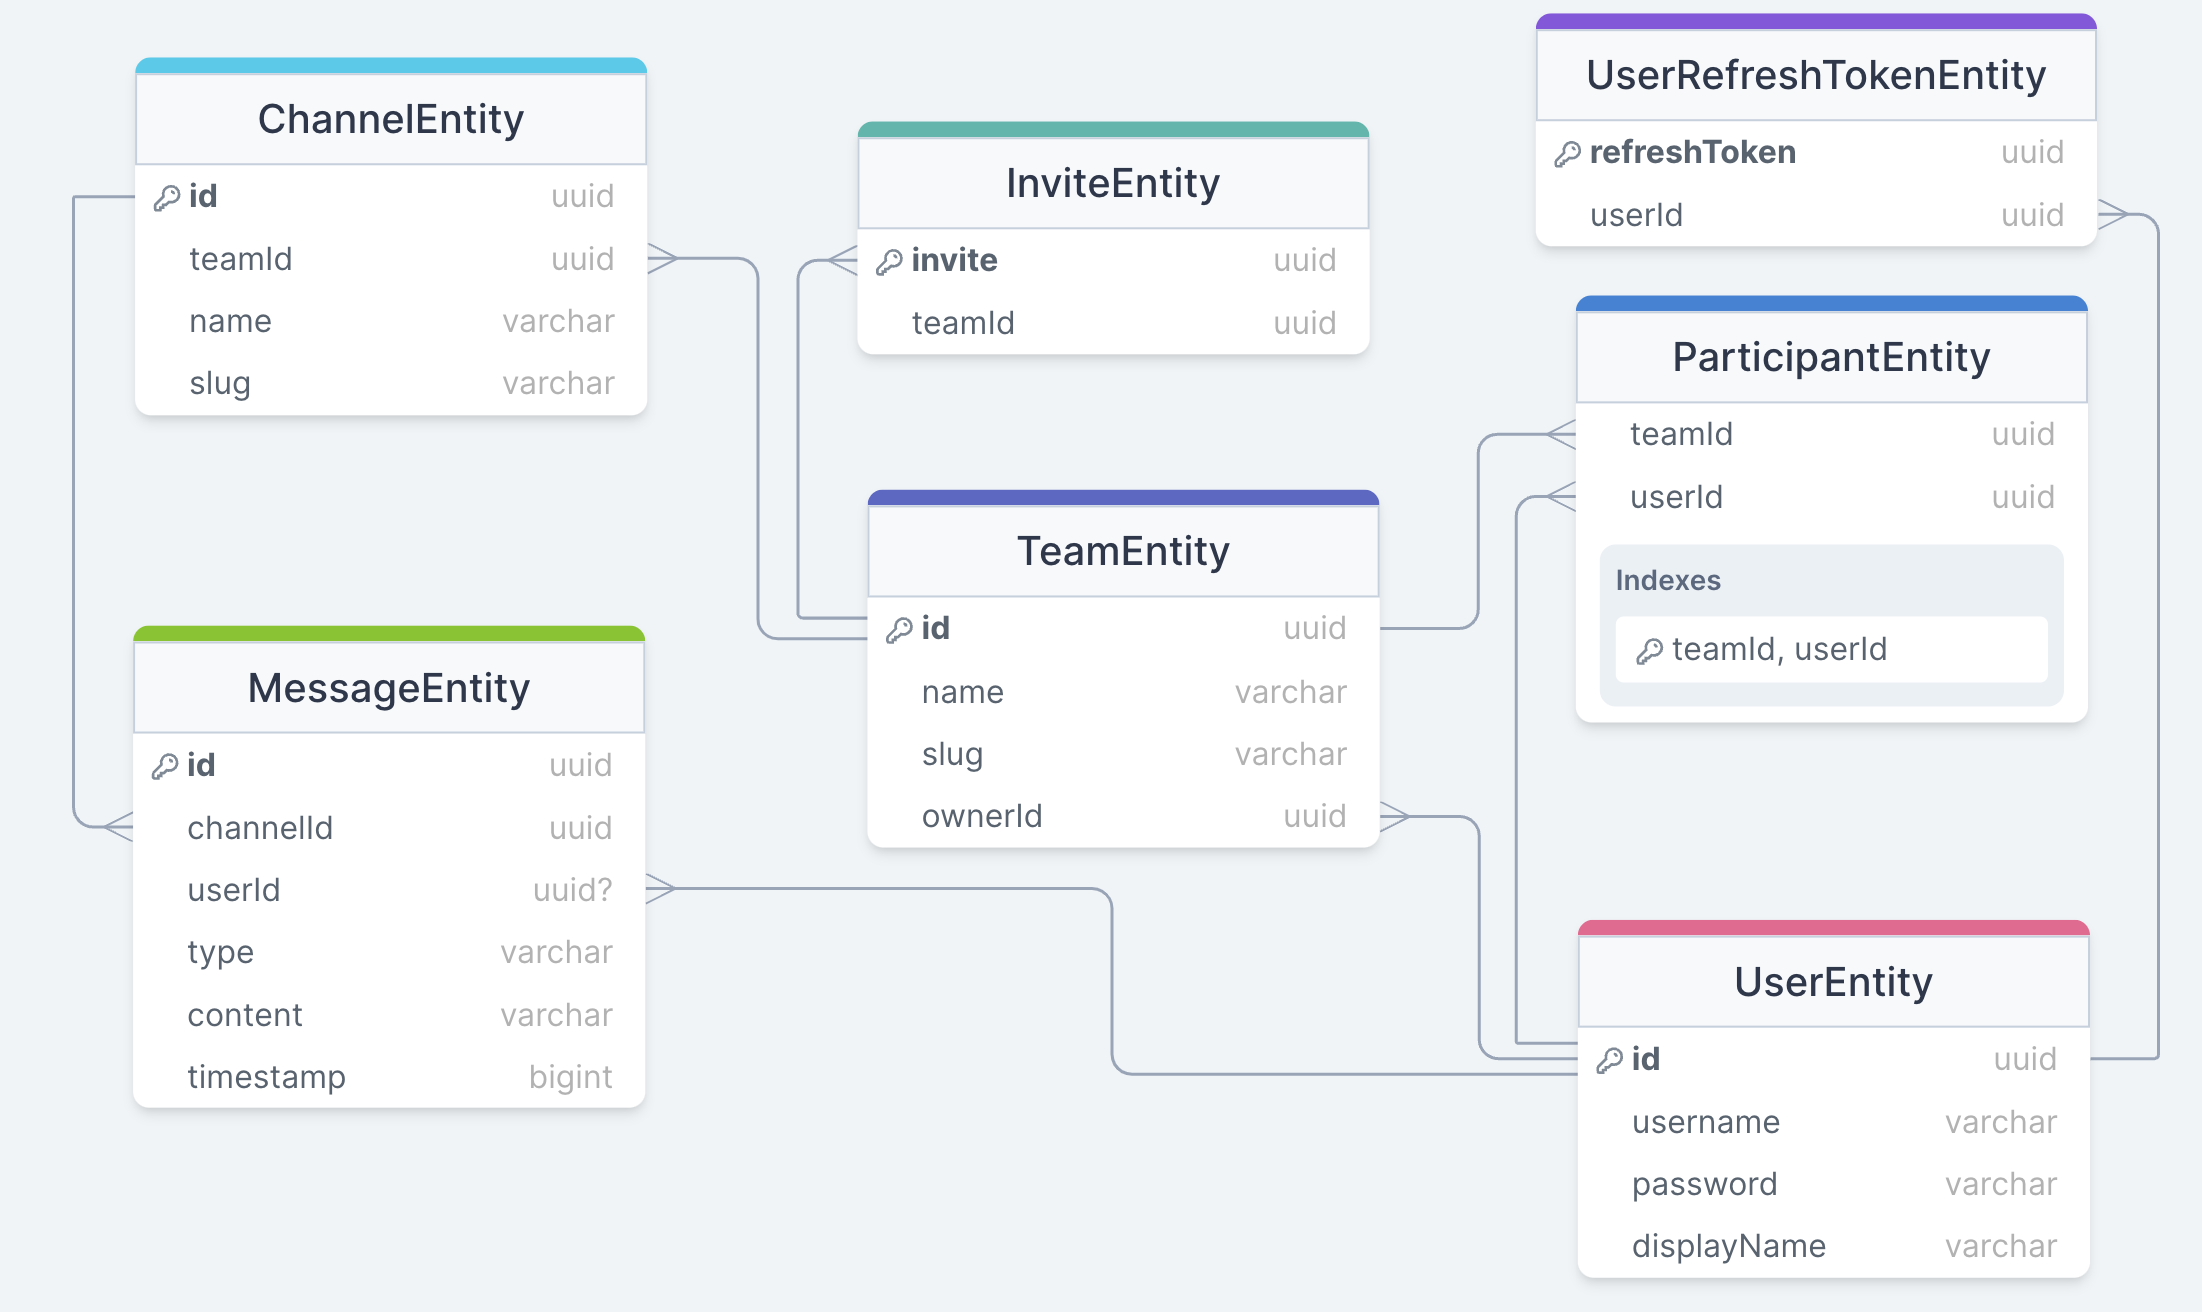
\includegraphics[scale=0.35]{./assets/db_schema.png}
  \caption{Datenbank-Schema}\label{fig:dbSchema}
\end{figure}

Für das Nutzerverwaltung werden zwei Tabellen benötigt, zum einen die
\emph{UserEntity} Tabelle als auch die \emph{UserRefreshTokenEntity} Tabelle.
Die \emph{UserEntity} Tabelle hält den Nutzer selbst. Dies beinhaltet den einen
Nutzernamen für den Login, ein Passwort, welches zuvor gehashed wird, und einen
Anzeigenamen für die Teilnehmerliste und Chatnachrichten. Die \emph{UserRefreshTokenEntity}
Tabelle wird zusätzlich benötigt, um die \emph{refreshTokens} für die spätere
Authentifikation zu speichern.

Die weiteren Tabellen werden zur Verwaltung der Teams und der Unterkomponenten gebraucht.
Die \emph{TeamEntity} Tabelle, speichert den Namen des Teams und einen \emph{slug},
welcher später im Browser für eine lesbare Identifikation in der URL verwendet wird. Ein
Team ist immer an einem Besitzer verknüpft. Um weitere Nutzer zu einem Team einzuladen,
werden die Einladungscodes in der \emph{InviteEntity} Tabelle gespeichert. Nach
einem erfolgreichen Beitritt zu einem Team wird die Zugehörigkeit über die \emph{ParticipantEntity}
Tabelle festgehalten, in der Nutzer zu Teams zugeordnet werden. Weiterhin die verschiedenen
Textkanäle in der \emph{ChannelEntity} Tabelle gespeichert und besitzen auch wie ein Team selbst,
\emph{slugs} für die Verwendung im Browser. Zuletzt gibt es noch eine Tabelle für die Textnachrichten.
In diesen wird der der Inhalt einer Nachricht, der Verfasser und ein Zeitstempel, wann die Nachricht
geschrieben wurde, persistiert. Für den Inhalt der Nachricht gibt es zwei Spalten die \emph{type}
und \emph{content} Spalte. Dies wurde dafür verwendet, um eine zukünftige Erweiterbarkeit vorzunehmen,
wo \zb{} auch neben einfachen Textnachrichten Bilder oder andere Nachrichtentypen gesendet werden können.

\subsection{Architektur}

Zur Entwicklung des Projektes wird noch die generelle Architektur für die
gesamte Applikation benötigt. Da es sich hier um eine Webapplikation handelt
wurde eine Client-Server-Architektur gewählt. Dies soll heißen, dass es einen
Server (im Folgenden auch \anf{Backend} genannt) gibt, welcher die Daten und
die Domänenlogik der Applikation hält. Dieser selbst bietet keine
Interaktivität für den Nutzer. Die Interaktivität kommt durch die einzelnen
Clients (im Folgenden auch \anf{Frontend} genannt), die die Nutzer bedienten
können Zustande. Da eine Webapplikation entwickelt wird, sind Clients die
Webbrowser der Benutzer. Ein Client bietet so die Interaktivität und
kommuniziert zum Erhalt der Daten und zur Manipulation dieser mit dem Server.

Der Server folgt dabei einer einfachen Schichtenarchitektur. In dieser werden
die Dienste einer Applikation in mehrere Schichten aufgebaut, welche aufeinander
aufbauen. So wird die Funktionalität der vorherigen Schicht verwendet, um diese
zu erweitern und eigene Funktionalität in einer hinzuzufügen.
(\vgl{}~\cite[\page{} 35]{layeredArch}) Dabei wurde das Backend in drei
Schichten gegliedert: die Datenschicht, die Businessschicht und die
Präsentationsschicht. Durch die Datenschicht werden wird ein Zugang zu den
Daten in der Datenbank und weiteren Persistenztechnologien ermöglicht.
Diese können durch die Schicht erhalten und manipuliert werden. In der Businessschicht
wird die eigentliche Applikationslogik erstellt. Dies beinhaltet \zb{} die Erstellung eines Nutzers
oder das Senden von Textnachrichten. Zuletzt bietet die Präsentationsschicht eine
REST-Schnittstelle für die Interaktivität des Frontends und eine zusätzliche Websocket-Schnittstelle,
um Echtzeit-Benachrichtigungen zu erhalten.

Das Frontend selbst wird durch eine Single Page Applikation (SPA) gebildet. In
dieser wird das User-Interface (UI) dynamisch komplett im Browser generiert.
Dafür wird eine minimale HTML-Datei ausgegeben, welche den gesamten Quelltext
für das Bilden des eigentlichen User-Interfaces und der Interaktion mit dem
Backend enthält. Der Client kann über asynchrone Request im Hintergrund Daten
vom Backend erhalten und die UI dementsprechend anpassen. Bei Aktionen des
Nutzers, wie \zb{} dem Erstellen eines neuen Projektes oder seinem Login,
können auch Anfragen an den Server gesendet werden, um diese auszuführen.

\subsection{Verwendete Technologien}

Zuletzt sollten in der Konzeption, die verwendeten Technologien für das Projekt
beschrieben werden. Hierfür wird zwischen dem Frontend und Backend
unterschieden, da dafür zwei verschiedene Programmiersprachen verwendet wurden.
Die verwendete relationale Datenbank für die Datenhaltung wurde dabei schon in
dementsprechenden Kapitel beschrieben.

Für die Entwicklung des Backends wurde die Programmiersprache Kotlin einer Sprache,
die auf der JVM verwendet werden kann, und deren Ökosystem verwendet. Die wichtigsten
Pakete waren hierfür: \emph{sqldelight}~\cite{sqldelight}, \emph{ktor}~\cite{ktor}
und \emph{dagger}~\cite{dagger} zusammen mit \emph{anvil}~\cite{anvil}. \emph{sqldelight}
bietet dafür einen Typsicheren Zugriff zur Datenbank, welche über Quelltext-Generation geschieht.
Durch \emph{ktor} konnte die REST-Schnitstelle als auch das Behandeln von Websocket-Verbindungen
für die Präsentationsschicht implementiert werden. Zuletzt konnte über die Bibliothek
\emph{dagger} und dem Erweiterungspaket \emph{anvil} Paket, eine automatische Dependency-Injection
für die Verbindung der einzelnen Schichten und deren Diensten ermöglicht werden.

Das Frontend wurde mithilfe von TypeScript und der UI-Bibliothek
\emph{SolidJS}~\cite{solidjs} entwickelt. Dabei handelt es sich um eine
komponentenbasierte UI-Bibliothek, durch die einzelne UI-Elemente mithilfe von
einfachen Funktionen beschrieben werden können. Neben dieser wurde zwei
kleinere Bibliothek, welche die Funktionalität von \emph{SolidJS} erweitern,
verwendet.
